\documentclass[twoside,10pt,a4paper]{article}
\usepackage[utf8]{inputenc}
\usepackage[english]{babel}
\usepackage{amsmath}
\usepackage{amsfonts}
\usepackage{amssymb}
\usepackage{graphicx}

\usepackage[left=2cm,right=2cm,top=2cm,bottom=3cm]{geometry}
\usepackage{fancyvrb}
\usepackage{listings}
\usepackage{xparse}
\usepackage{tikz} % ajout de dessins LaTeX
\usepackage{graphicx}
\usepackage{float}  % alignement des figures
\usepackage{fancyhdr}
\usepackage{enumitem}
\usepackage{verbatim}
\usepackage{xcolor}

\usepackage{caption}
\usepackage{subcaption}

\pagestyle{fancy} %fancyhdr
	\fancyhf{} %fancyhdr
	\renewcommand{\sectionmark}[1]{\markboth{#1}{}}
	\fancyhead[R]{NLDCI Set 4 Questions} %INSERT TITLE HERE FOR fancyhdr
	\fancyhead[L]{\nouppercase{\leftmark}} %fancyhdr
	\cfoot{\thepage} %fancyhdr
	\setlength{\headheight}{35pt}
	\setlength{\parindent}{0pt}
	
	\definecolor{MyBlue}{HTML}{4A90E2}
	\definecolor{MyRed}{HTML}{D0021B}
	\definecolor{MyGreen}{HTML}{7ED321} % Same color use in Mathcha

\begin{titlepage}
\title{\huge \textbf{Nonlinear Dynamics \& Chaos I \\ \Large Exercice Set 4 Questions}}	%TITLE
\author{ }		%AUTHOR
\date{ }	%DATE

\end{titlepage}


\begin{document}

\maketitle

\section*{Question 1}
Consider the discrete dynamical system
\begin{align*}
	x_{n+1} &= Ax_n + f(x_n, y_n), \\
	y_{n+1} &= By_n + g(x_n, y_n),
\end{align*}
where $x_n \in \mathbb{R}^c$, $y_n \in \mathbb{R}^d$, $A \in \mathbb{R}^{c \times c}$, $B \in \mathbb{R}^{d \times d}$; $f$ and $g$ are $C^r$ functions with no linear terms. Assume that all eigenvalues of $A$ have modulus one, and none of the eigenvalues of $B$ have modulus one. Then the linearized system at the origin admits a center subspace $E^c$ aligned with the $x$-coordinate plane.

\begin{enumerate}[label=(\alph*)]
	\item Derive a general algebraic equation for the center manifold $W^c$, which is known to exist by a theorem analogous to the center manifold theorem for continuous dynamical systems.
	\item Find a cubic order approximation for the center manifold of the discrete system
	\begin{align*}
		x_{n+1} &= x_n + x_ny_n, \\
		y_{n+1} &= \lambda y_n - x_n^2,
	\end{align*}
	where $\lambda \in (0,1).$
	\item Reduce the dynamics to the center manifold and determine the stability of the origin. Verify your results by a numerical simulation of a few initial conditions near the origin.
\end{enumerate}

\section*{Question 2}
Construct a cubic-order local approximation for the unstable manifold of the hyperbolic fixed point of the pendulum equation
\begin{equation*}
	\ddot{x} + \sin(x) = 0.
\end{equation*}

\section*{Question 3}
Consider the discrete dynamical system
\begin{equation*}
	\begin{cases}
		x_{n+1} = x_n + x_ny_n \\
		y_{n+1} = \frac{1}{2}y_n - x_n^2
	\end{cases}
\end{equation*}
Let $h:(-\varepsilon, \varepsilon) \longrightarrow \mathbb{R}$ be the local graph of the \underline{center manifold} around $(0,0)$. $(0 < \varepsilon \ll 1)$. Find the expression that $h$ satisfies.

\begin{enumerate}[label=(\alph*)]
	\item $ \displaystyle h(x + h(x)) - \frac{1}{2}h(x) = x^2 $
	\item $ \displaystyle h(x + h(x)) - \frac{1}{2}h(x) = -x^2 $
	\item $ \displaystyle h(x + xh(x)) - \frac{1}{2}h(x) = x^2 $
	\item $ \displaystyle h(x + xh(x)) - \frac{1}{2}h(x) = -x^2 $
\end{enumerate}

\section*{Question 4}
Consider the following dynamical system
\begin{equation*}
	\begin{cases}
		\dot{x} = xy \\
		\dot{y} = -y + x^2
	\end{cases}
\end{equation*}
Which expression describes the reduced dynamics on the center manifold?

\begin{enumerate}[label=(\alph*)]
	\item $ \dot{x} = x^3(1 - 2x^2) + \mathcal{O}(x^5) $
	\item $ \dot{y} = y^3(1 - 2y^2) + \mathcal{O}(y^5) $
	\item $ \dot{x} = x^3(1 + 2x^2) + \mathcal{O}(x^5) $
	\item $ \dot{y} = y^3(1 + 2y^2) + \mathcal{O}(y^5) $
\end{enumerate}

\section*{Question 5}
Consider the following dynamical system
\begin{equation*}
	\begin{cases}
		\dot{x} = -x^3 \\
		\dot{y} = -y
	\end{cases}
\end{equation*}
Let $y = h(x)$ be the graph of the center manifold of $(0,0)$. Which of the following expressions is accurate ?

\textit{Hint}: $ \displaystyle \frac{dy}{dx} = \frac{\dot{y}}{\dot{x}} = \frac{y}{x^3} $

\begin{enumerate}[label=(\alph*)]
	\item The dynamical system has a unique center manifold with $ \displaystyle h(x) = e^{-\frac{1}{2x^2}} $
	\item The dynamical system has a unique center manifold with $ \displaystyle h(x) = e^{-\frac{1}{x^2}} $
	\item The dynamical system has infinitely many center manifolds with $ \displaystyle h(x) = \begin{cases}
		ae^{-\frac{1}{2x^2}} & x < 0 \\
		0 & x = 0 \\
		be^{-\frac{1}{2x^2}} & x > 0
	\end{cases} \;\; \forall a,b \in \mathbb{R}$
	\item The dynamical system has infinitely many center manifolds with $ \displaystyle h(x) = \begin{cases}
		ae^{-\frac{1}{x^2}} & x < 0 \\
		0 & x = 0 \\
		be^{-\frac{1}{x^2}} & x > 0
	\end{cases} \;\;  \forall a,b \in \mathbb{R}$
\end{enumerate}

\section*{Question 6}
The phase portrait of four planar dynamical systems are shown below. In which case is the origin \underline{not} Lyapunov stable?

\begin{enumerate}[label=(\alph*)]
	\item 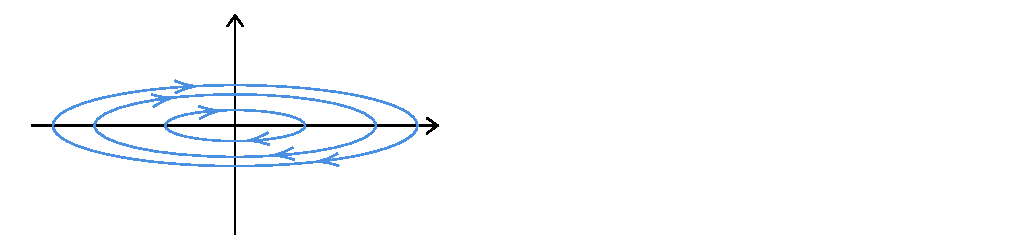
\includegraphics[scale=0.8]{Graphics/MCQ1_figures/Q17D01.pdf}
	\item 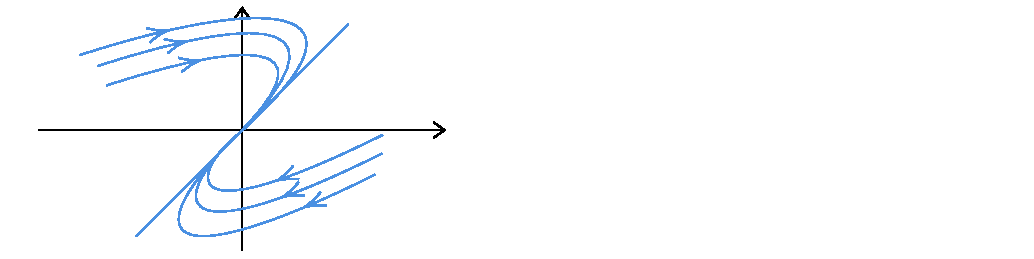
\includegraphics[scale=0.8]{Graphics/MCQ1_figures/Q17D02.pdf}
	\item 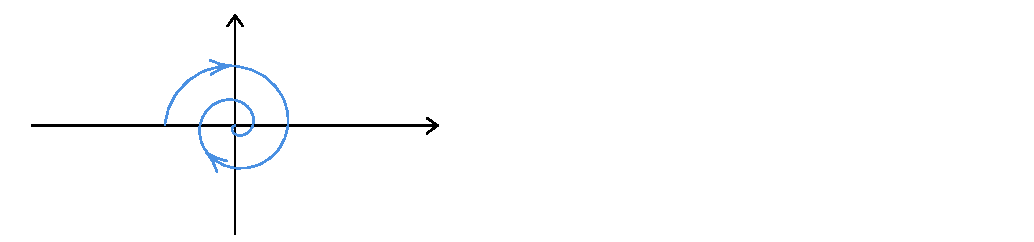
\includegraphics[scale=0.8]{Graphics/MCQ1_figures/Q17D03.pdf}
	\item 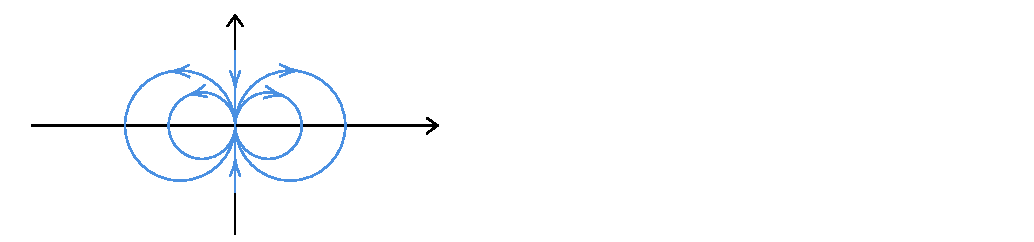
\includegraphics[scale=0.8]{Graphics/MCQ1_figures/Q17D04.pdf}
\end{enumerate}

\section*{Question 7}
Consider the dynamical system below
\begin{equation*}
	\dot{x} = |x|^2 (Ax + f(x))
\end{equation*}
where , $x \in \mathbb{R}^n, \; f \in C^1, \; A \in \mathbb{R}^{n \times n}, \; f = \mathcal{O}(|x|^2)$ and the matrix $A$ has precisely one pair of purely imaginary eigenvalues, and $(n - 2)$ eigenvalues with negative real parts.

Which of the following statements are true?

\begin{enumerate}[label=(\alph*)]
	\item The origin $x = 0$ is unstable.
	\item $ \dim(W^c(0)) = 2 $
	\item$ \dim(W^c(0)) = n $
	\item None of the above
\end{enumerate}



\end{document}